\subsection{Hammer Projektion}
\label{sec:Hammer}
Die Hammer Projektion ist wie die Mollweiden Projektion eine flächentreue Projektion.
Bei der Hammer Projektion wird die Erden ebenfalls als Oval dargestellt. Allerdings werden die Breitenkreise im Gegensatz zur Mollweiden Projektion als Ellipsen dargestellt, dadurch ist die Verzerrung an den Rändern nicht so stark. Nachteil bei dieser Art der Darstellung ist, dass die Erde an den Polen gestaucht wird.\\

\begin{figure}[hbtp]
\centering
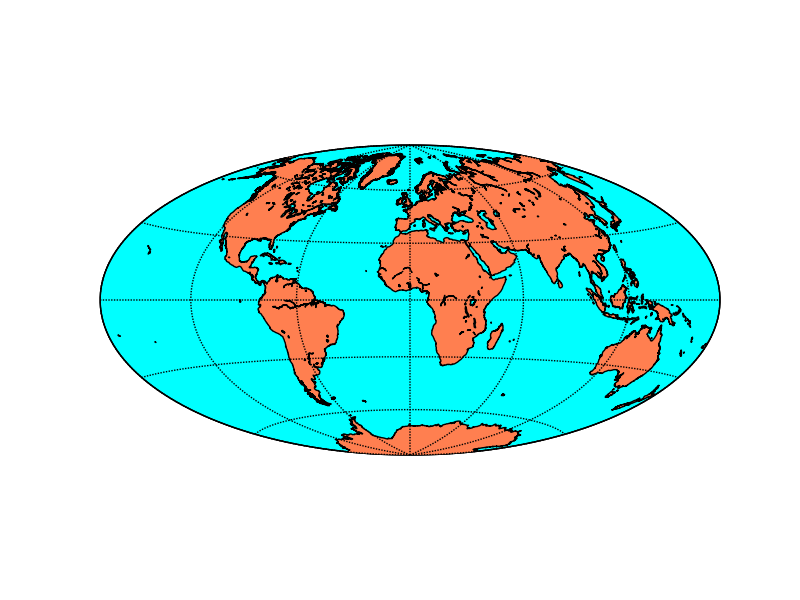
\includegraphics[scale=0.5,origin=c]{/Users/student/seminar/Kartendarstellungen/seminar/hammer} \caption{Hammer Projektion}
\end{figure}
\newpage 